%%%%%%%%%%%%%%%%%%%%%%%%%%%%%%%%%%%%%%%%%
% Simple Sectioned Essay Template
% LaTeX Template
%
% This template has been downloaded from:
% http://www.latextemplates.com
%
% Note:
% The \lipsum[#] commands throughout this template generate dummy text
% to fill the template out. These commands should all be removed when 
% writing essay content.
%
%%%%%%%%%%%%%%%%%%%%%%%%%%%%%%%%%%%%%%%%%

%----------------------------------------------------------------------------------------
%	PACKAGES AND OTHER DOCUMENT CONFIGURATIONS
%----------------------------------------------------------------------------------------

\documentclass[12pt]{article} % Default font size is 12pt, it can be changed here
\usepackage{hyperref}
\usepackage{geometry} % Required to change the page size to A4
\usepackage{graphicx}
\geometry{a4paper} % Set the page size to be A4 as opposed to the default US Letter

\usepackage{graphicx} % Required for including pictures

\usepackage{float} % Allows putting an [H] in \begin{figure} to specify the exact location of the figure
\usepackage{wrapfig} % Allows in-line images such as the example fish picture
\usepackage{listings}
\usepackage[usenames,dvipsnames]{color} % Required for custom color
\linespread{1.2} % Line spacing

\definecolor{MyDarkGreen}{rgb}{0.0,0.4,0.0} % This is the color used for comments
\lstloadlanguages{C++} % Load C++ syntax for listings, for a list of other languages supported see: ftp://ftp.tex.ac.uk/tex-archive/macros/latex/contrib/listings/listings.pdf
\lstset{language=Perl, % Use Perl in this example
        frame=single, % Single frame around code
        basicstyle=\small\ttfamily, % Use small true type font
        keywordstyle=[1]\color{Blue}\bf, % Perl functions bold and blue
        keywordstyle=[2]\color{Purple}, % Perl function arguments purple
        keywordstyle=[3]\color{Blue}\underbar, % Custom functions underlined and blue
        identifierstyle=, % Nothing special about identifiers                                         
        commentstyle=\usefont{T1}{pcr}{m}{sl}\color{MyDarkGreen}\small, % Comments small dark green courier font
        stringstyle=\color{Purple}, % Strings are purple
        showstringspaces=false, % Don't put marks in string spaces
        tabsize=5, % 5 spaces per tab
        %
        % Put standard Perl functions not included in the default language here
        morekeywords={rand},
        %
        % Put Perl function parameters here
        morekeywords=[2]{on, off, interp},
        %
        % Put user defined functions here
        morekeywords=[3]{test},
       	%
        morecomment=[l][\color{Blue}]{...}, % Line continuation (...) like blue comment
        numbers=left, % Line numbers on left
        firstnumber=1, % Line numbers start with line 1
        numberstyle=\tiny\color{Blue}, % Line numbers are blue and small
        stepnumber=5 % Line numbers go in steps of 5
}

% Creates a new command to include a perl script, the first parameter is the filename of the script (without .pl), the second parameter is the caption
\newcommand{\cppcode}[2]{
\begin{itemize}
\item[]\lstinputlisting[caption=#2,label=#1]{#1.pl}
\end{itemize}
}


\graphicspath{{./Pictures/}} % Specifies the directory where pictures are stored
\usepackage{amsmath}
\usepackage{centernot}
\usepackage[T1]{fontenc}
\newcommand{\tab}{\hspace*{2em}}
\begin{document}

%----------------------------------------------------------------------------------------
%	TITLE PAGE
%----------------------------------------------------------------------------------------

\begin{titlepage}

\newcommand{\HRule}{\rule{\linewidth}{0.5mm}} % Defines a new command for the horizontal lines, change thickness here

\center % Center everything on the page

\textsc{\LARGE Columbia University}\\[1.5cm] % Name of your university/college
\textsc{\Large Computer Science Department}\\[0.5cm] % Major heading such as course name
\textsc{\large COMS W4115 Programming Languages and Translators}\\[0.5cm] % Minor heading such as course title

\HRule \\[0.4cm]
{ \huge \bfseries Matcab: Matrix Manipulation Language}\\[0.4cm] % Title of your document
\HRule \\[1.5cm]

\begin{minipage}{0.4\textwidth}
\begin{flushleft} \large
\emph{Author:}\\
Cheng Xiang \\ Yu Qiao \\ Ran Yu \\ Tianchen Yu % Your name
\end{flushleft}
\end{minipage}
~
\begin{minipage}{0.4\textwidth}
\begin{flushright} \large
\emph{Supervisor:} \\
Prof. Stephen A. Edwards\ % Supervisor's Name
\end{flushright}
\end{minipage}\\[4cm]

{\large \today}\\[3cm] % Date, change the \today to a set date if you want to be precise



\vfill % Fill the rest of the page with whitespace

\end{titlepage}

%----------------------------------------------------------------------------------------
%	TABLE OF CONTENTS
%----------------------------------------------------------------------------------------

\tableofcontents % Include a table of contents

\newpage % Begins the essay on a new page instead of on the same page as the table of contents 

%----------------------------------------------------------------------------------------
%	INTRODUCTION
%----------------------------------------------------------------------------------------

\section{Introduction} % Major section

The MatCab is a programming language that simplifies and accelerates matrix manipulations. It is a C-style language that particularly aims at easier and faster matrix computing for programmers. Matrix computing is one of the most common linear algebra operations used in scientific computation. Operations like image processing and data mining both require considerable amount of highly efficient matrix calculations. For example, in the multi-dimensional regression, a basic algorithm in Machine Learning, we need to compute the inverse of the matrix. Instead of writing multiple lines to implement the inverse function and maybe error-prone due to the unfamiliar with inverse concept. Our MatCab language, however, provides an easy way to apply basic arithmetical operation to matrices. Like that you can simply type 'A"' to get the inverse matrix of A. And its C-like syntax can help C programmers get rid of the burden of hundreds of lines of c-code for matrix computing, making the computation simple, compact and easy to read. \\
MatCab simplifies matrix processing, through domain-specific data types and operators. A basic data type in MatCab is a $FloatMat$, which is a 2-dimension matrix consist of float numbers. And $FloatMat$ support  various basic Matrix computation, such as $inverse,~,transpose,~,convolution,~\dots$ and etc.\\
With the feature of matrix manipulation, MatCab can be widely use in programming about calculation. The intuitive, robust and portable MatCab can do a lot in programming. 
%---------------------------------------------
%	Language Tutorial
%---------------------------------------------
\section{Language Tutorial}
\subsection{General Purpose Programs}
At the beginning, I would like to demonstrate our MatCab language with a simple general purpose program that calculates the greatest common divisor.

\begin{lstlisting}[firstline=1,lastline=30]
int gcd(int a, int b) {
    while (a != b) {
        if (a > b) 
            a = a - b;
        else
            b = b - a;
        endif;
    }
    return a;
}

int entry() {
    int a;
    a = gcd(2, 14);
    print(a);
}

}
\end{lstlisting}

In this gcd.mcb program, language features like function declaration, function call( gcd(2, 14) ), while loop, if-else branching, variable declaration are presented. More precise syntax specification is given in later part of this report.

\subsection{MAE}

In order to demonstrate the simplicity in syntax of matrix manipulations, the code for mae.mcb program is given as below. MAE stands for Mean-Average-Error. This is an indicator of the quality of decomposing one huge matrix into approximately the product of two matrices with much smaller dimension.

\begin{lstlisting}[firstline=1,lastline=30]
int entry() {
    int i;
    int j;
    int cnt;
    floatMat A;
    floatMat B;
    floatMat C;

    Init B[20][4];
    Init C[4][10];
    Init A[20][10];

    B = [[
        1, 2, 3, 4  ?
        7, 3, 9, 1  ?
        5, 6, 7, 3  ?
        3, 9, 1, 4  ?
        8, 3, 5, 3  ?
        6, 3, 2, 7  ?
        2, 8, 5, 3  ?
        4, 2, 9, 4  ?
        6, 3, 8, 4  ?
        7, 9, 5, 2  ?
        3, 8, 6, 9  ?
        3, 0, 3, 1  ?
        4, 2, 2, 7  ?
        1, 6, 8, 7  ?
        3, 0, 4, 3  ?
        6, 5, 7, 2  ?
        2, 7, 7, 3  ?
        5, 3, 6, 9  ?
        2, 5, 5, 3  ?
        3, 5, 6, 9  ]];

    C = [[
        6, 3, 4, 7, 9, 5, 3, 1, 3, 3 ?
        8, 4, 2, 4, 5, 7, 9, 0, 6, 7 ?
        9, 3, 2, 1, 4, 8, 9, 8, 5, 3 ?
        3, 4, 4, 5, 2, 7, 5, 8, 3, 2 ]];

    A = [[
        64, 39, 28, 33, 39, 68, 69, 58, 42, 33 ?
        150,64, 56, 75, 116,135,134,87, 87, 74 ?
        150,72, 58, 81, 109,144,147,85, 95, 84 ?
        111,64, 48, 78, 84, 114,119,43, 80, 83 ?
        126,63, 60, 88, 113,122,111,77, 76, 66 ?
        99, 64, 62, 91, 91, 116,98, 78, 67, 59 ?
        130,65, 46, 66, 84, 127,138,66, 88, 83 ?
        133,63, 54, 65, 90, 134,131,108,81, 61 ?
        144,70, 62, 82, 109,143,137,102,88, 71 ?
        165,80, 64, 100,132,155,157,63, 106,103?
        163,95, 76, 104,109,182,180,123,114,101?
        48, 22, 22, 29, 41, 46, 41, 35, 27, 20 ?
        79, 54, 52, 73, 68, 99, 83, 76, 55, 46 ?
        147,79, 60, 74, 85, 160,164,121,100,83 ?
        63, 33, 32, 40, 49, 68, 60, 59, 38, 27 ?
        145,67, 56, 79, 111,135,136,78, 89, 78 ?
        140,67, 48, 64, 87, 136,147,82, 92, 82 ?
        135,81, 74, 98, 102,157,141,125,90, 72 ?
        106,53, 40, 54, 69, 106,111,66, 70, 62 ?
        139,83, 70, 92, 94, 161,153,123,96, 80 ]];

    A = B * C - A;
    cnt = 20 * 10;
    
    print(sum(A, 0, 0, 19, 9) / (20 * 10));
}
\end{lstlisting}

In this program you may see language features including matrix multiplication operation (simply achieved by overriding * operator) , matrix subtraction operation (unlike C-style syntax that iterates through the 2-dimensional array, the difference of corresponding elements of two matrix of same type and dimensions can be directly returned using - operator).

\subsection{Gaussian Filter}


\subsection{Compiling and Running Your Program}
First make the MatCab compiler by running \begin{verbatim}make\end{verbatim}. Then use  \begin{verbatim}./matcab -e < gcd.mcb\end{verbatim} to compile and run your program. If you just want to compile and do not want to run the program, use ``-e'' parameter. If you want to view the AST of your program, use the ``-a'' parameter.

%----------------------------------------------------------------------------------------
%	MAJOR SECTION 1
%----------------------------------------------------------------------------------------
\section{Language Reference Manual}
\subsection{Program Definition} % Major section
A MatCab Program consists of any number of global variable declarations and several function definitions. The compiler will find the function with function name ``entry'' and start executing the program from this entry function. There’s no requirement for the order of such variable definitions or function definitions. Users can arrange the order of appearance of them in any way they would like to. Our compiler is able to fetch the right function that a user is pointing to no matter this function is defined before or after the definition of entry function.

There are two now existing limitation about MatCab programs. The first is that now the compiler cannot process arguments given from command line, which means that the behavior of one MatCab program is pretty determinant and predictable, lacking some extend of flexibility. The second flaw of our current implementation of MatCab language is that now our compiler will accept only one input source program. If a user would like to take advantage of some existing implemented function, he/she would have to copy the code of such functions to the new source MatCab program.

Each variable declaration consists of a type specification and a variable name designation. Each function definition is the combination of return type specification, function name designation, formal list declaration and function body specification. The rules for naming a variable or a function are given in later discussion of this MatCab language specification document. Formal list of a function may contain none, one or more than one arguments (with the only exception of entry function that can take in no arguments). MatCab programmers are required to explicitly specify the type of the formal arguments. The function body is simply a list of MatCab language statements. Local variables are declared at the head of the function body. Though the order of variable declarations and function definitions within the source program is of no limit, all the declarations of variables have to appear before any other statements within that function body scope.

Please refer to the gcd.mcb program in section 2.1. This program calculates the greatest common divisor of two integers. A function named gcd, with return type int, is declared before the entry function. And it is later called by the entry function to give out the greatest common divisor of 2 and 14.


\subsection{Lexical Conventions} % Major section

There are six kinds of tokens: comments, identifiers, keywords, constants, strings, and operators. Comments, blanks, tabs, tabs, new lines and are ignored. The token is recognized until the parser sees a separator.
%------------------------------------------------
\subsubsection{Comments} 
Program segments enclosed in the ``/*'' and ``*/'' are considered as the comments of MatCab program. Our compiler will simply ignore and discard such code segments. No nested ``/*''-``*/'' pairs are allowed, otherwise a syntax error will occur.

\begin{center}
\emph{/*This is a line of comment.*/}
\end{center}

%------------------------------------------------
\subsubsection{Identifiers}
An identifier is used to distinguish one variable or function from another. It consists of a sequence of letters and numbers, which are demanded to start with a letter. The identifiers are case-sensitive, i.e. Seen by the compiler, ``move'' and ``Move'' are different identifiers.

\begin{center}
\emph{foo,bar,BAR}
\end{center}

%------------------------------------------------
\subsubsection{Keywords} 
Like almost every other programming language on earth, MatCab has a series of reserved keywords. MatCab programmers cannot use them to name their variables nor functions. They are serving for different purposes. Names of built-in types, built-in functions are preserved. Some keywords are for flow-control purposes.
\begin{center}
\emph {Keyword  \ensuremath{\rightarrow} 
   \big| float \big| int    \big| floatMat \big| intMat
  \big| intRowVec \big| floatRowVec   \big| intColVec \big| floatColVec  
  \big| sum \big| init  
       \big| if \big| else \big| endif \big| for \big| while \big| entry 
       \big| true \big| return \big| true \big| false 
}
\end{center}

%------------------------------------------------
\subsubsection{Constants} 
MatCab language has two primitive types: integers and floats. Thus the constant literals in MatCab are either integer literals or float literals. An integer literal is a series of number digits. A float constant contains an integer part, a decimal point, and a fraction part.
%------------------------------------------------

%\subsubsubsection{Numeric Constants} 
A numeric constant can be an integer constant, a float constant.
The integer is a series of numbers. The float constant contains an integer part, a decimal point, a fraction part and a character `f'.

\begin{center}
\emph {Numeric Constant \ensuremath{\rightarrow} Integer Constant \big| Float Constant}

\emph {Integer Constant \ensuremath{\rightarrow} {[}0-9{]}+}

\emph {Float Constant \ensuremath{\rightarrow} {[}0-9{]}+ . {[}0-9{]}+ `f'}
\end{center}


%------------------------------------------------
\subsection{Operators} 
Being a language that aiming at simplifies the syntax of carrying out arithmetic operations, especially matrix calculations, the operators defined in the MatCab language is of great importance.

\begin{table}
\centering
\caption{Operators}
\begin{tabular}{|p{1cm}|p{12cm}|} \hline
Symbol & Explanation\\ \hline
+, - &  Binary operator that performs addition/subtraction operation. Operands could be int-int, int-float, float-int, float-float, matrix-int, matrix-float, int-matrix, float-matrix, and matrix-matrix pairs \\ \hline
-   & Unary operator that gives the value with opposite sign of given constant literal or variable. Operand is a integer or a float number. \\ \hline
*, /  &  Binary operator that performs multiplication/division operation. Operands could be int-int, int-float, float-int, float-float, matrix-int, and matrix-float pairs \\ \hline
\% &  Binary operator that performs modular operation. Operands could be int-int pairs. \\ \hline
>, >=, <, <= ,==, != &  Binary operator that performs greater-than/no-less-than/less-than/no-greater-than/equals/not-equals comparisons. Operands could be int-int or float-float pairs  \\ \hline
** & Binary operator that performs convolution operation. Operands are matrix-matrix pairs. \\ \hline
‘   &Unary operator that performs transposition operation. Operand is a matrix. \\ \hline
“  & Unary operator that performs matrix-inverse calculation. Operand is a matrix. \\ \hline
\&\&, || & Binary operator that performs AND/OR Boolean operation. Operands are Boolean expressions.\\ \hline
!   & Unary operator that performs NOT Boolean operation. Operand is Boolean expression.\\ \hline

\end{tabular}
\end{table}

The precedence and associativity are in correspondence with the equivalent operators in other common general purpose programming language, C for instance.
%------------------------------------------------
\subsection{Types} 
MatCab now supports integer and float variables as primitive type variables. As of the matrix part, all elements of a matrix must be float numbers.
%------------------------------------------------

%------------------------------------------------
\subsection{Expressions}
Here the definition of MatCab expressions follows the steps in C Language Reference Manual defining expressions.

%------------------------------------------------
\subsubsection{Assignment expressions}
Assignment expressions are of form:
\begin {center}
Identifier AssignOperator expr
\end {center}

%------------------------------------------------
\subsubsection{ Built-in function call expressions}
Calling a built-in function with argument of a matrix is identified as an expression by our parser. For example, | A | is asking for the determinant of the matrix A. Such function calls are:
\begin {center}
| expr |

tr ( expr )

submat ( expr, expr, expr, expr, expr )

sum ( expr, expr, expr, expr, expr )

\end {center}

%------------------------------------------------
\subsubsection{User defined function calls}
User defined functions are called in the same manner as in built-in function calls.User defined functions are called in the same manner as in built-in function calls.
\begin {center}
Identifier ( argument\_list\_optional )
\end {center}

%------------------------------------------------
%\subsubsection{Arithmetic expressions}
%Applying arithmetic operators to expressions generates new expressions. They are of form:
%\begin {center}
%expr  binary\_operator expr
%expr right\_hand\_side\_unary\_operator
%left\_hand\_side\_unary\_operator expr
%\end {center}
%------------------------------------------------
\subsubsection{Declarations}
There are two kinds of declaration statements in MatCab: variable declarations and function declarations.
Variable declarations are of form: \begin{center}Type Identifier ;\end{center}
Function declarations are of form: \begin{center}Type Identifier ( formal\_list ) { function\_body }\end{center}
A function may take in no arguments, which means that the formal list is an optional part for a function declaration. The function body consists of local variable declarations and statements. Any local variables being used within this function body must be declared first before any of the statements. The statements are parsed and executed line by line.

%------------------------------------------------
\subsection{Statements}
Statements in MatCab language can be classified as four types: simple statements, grouped statements, matrix initialization statements and flow control statements.

A single semicolon or an expression followed by a semicolon are parsed as simple statements.

A series of statements enclosed by a pair of curly brackets are considered as one single statement. It is like:
\begin{center} { statement-1; statement-2;... statement-n; } \end{center}

Before applying operations to a declared matrix, it must be initialized with its dimensions first. The matrix initialization statements are of form:
\begin{center} Init Identifier [ expr ] [ expr ]  \end{center}
In which the first expression specifies the number of rows of this matrix, and the second expression specifies the number of columns of this matrix.

\subsection{Flow Control Statements}
Basic flow control statements including if, ifelse, for, while, return statements are supported in MatCab. The formal definition is given as below:
\begin{center} 
If ( Boolean\_expression ) statement endif ;

If ( Boolean\_expression ) statement else statement endif ;

For ( expression; Boolean\_expression; expression ) statement

While ( Boolean\_expression ) statement

Return expression ;
\end{center}

%------------------------------------------------
\subsection{Program Definition}
A MatCab program consists of several definition statements and exactly one entry point. The entry point itself is a function declaration with a specified form:
\begin{verbatim}
program
        /* Global variables; Function declarations; Entry point. */
        : { [], [] }
        | program VarDecl  { ( $2 :: fst $1 ), snd $1 }
        | program FuncDecl { fst $1, ( $2 :: snd $1 ) }
;

VarDecl_list
        : /* nothing */ { [] }
        | VarDecl_list VarDecl { $2 :: $1 }
;

VarDecl
        : Type IDENTIFIER SEMICOLON { { var_type = $1; var_name = $2 } }
;

FuncDecl
        : Type IDENTIFIER LPAREN formal_list_opt RPAREN LBRACE 
        VarDecl_list Statement_list RBRACE 

formal_list_opt
        : { [] }
        | formal_list { $1 }

formal_list
        : Type IDENTIFIER formal_list_rest { { var_type = $1; var_name = $2; } :: $3 }
;

formal_list_rest
        : /* nothing */ { [] }
        | COMMA formal_list { $2 }
;

Type
        : INT { Int }
        | FLOAT { Float }
        | INTROWVEC { IntRowVec }
        | FLOATROWVEC { FloatRowVec }
        | INTCOLVEC { IntColVec }
        | FLOATCOLVEC { FloatColVec }
        | INTMAT        { IntMatrix }
        | FLOATMAT      { FloatMatrix }
;

Statement_list
        : /* nothing */ { [] }
        | Statement_list Statement { $2 :: $1 }
;

Statement
        : expr SEMICOLON { Expr($1) }
        | SEMICOLON { Empty }
        | LBRACE Statement_list RBRACE { Block($2) }
        | IF LPAREN Bool_expr RPAREN Statement ELSE Statement ENDIF SEMICOLON
        | IF LPAREN Bool_expr RPAREN Statement ENDIF SEMICOLON 
        | FOR LPAREN expr SEMICOLON Bool_expr SEMICOLON expr RPAREN Statement
        | WHILE LPAREN Bool_expr RPAREN Statement 
        | EXPORT LPAREN IDENTIFIER RPAREN SEMICOLON
        | IDENTIFIER ASSIGN IMPORT LPAREN IDENTIFIER RPAREN SEMICOLON
        | RETURN expr SEMICOLON 
        | INIT IDENTIFIER LBRACKET expr RBRACKET LBRACKET expr RBRACKET
;

data
        : FLOAT_LITERAL { Float_lit($1) }
        | INT_LITERAL { Int_lit($1) }
        | TRUE { Boolean($1) }
        | FALSE { Boolean($1) }
;

Int_Row
        : { [] }
        | expr { [$1] }
                | Int_Row COMMA expr { $3 :: $1 }

IntMat_Init
        : Int_Row { [List.rev $1] }
        | IntMat_Init QUES Int_Row { $1 @ [List.rev $3] }

IdList_opt
        : { [] }
        | IdList { $1 }

IdList
        : expr { [$1] }
        | IdList COMMA expr { $1 @ [$3] }

expr
        : data { $1 }
        | IDENTIFIER ASSIGN expr { VarAssign($1, $3) }
        | BAR expr BAR { Det($2) }
        | SLASH IntMat_Init BACKSLASH { Im_init($2) }
        | TRACE LPAREN expr RPAREN { Trace($3) }
        | SUBMAT LPAREN expr COMMA expr COMMA expr COMMA expr COMMA expr RPAREN 
        | SUM LPAREN expr COMMA expr COMMA expr COMMA expr COMMA expr RPAREN 
        | IDENTIFIER LBRACKET expr RBRACKET LBRACKET expr RBRACKET 
        | IDENTIFIER { Id($1) }
        | LPAREN expr RPAREN { $2 }
        | IDENTIFIER LPAREN IdList_opt RPAREN { Call($1, $3) }
        | expr TIMES expr { Binary_op($1, Times, $3) }
        | expr DIVIDES expr { Binary_op($1, Divides, $3) }
        | expr MODE expr { Binary_op($1, Mode, $3) }
        | expr MTIMES expr { Binary_op($1, Mtimes, $3) }
        | expr CONVOLUTION expr { Binary_op($1, Convolution, $3) }
        | expr PLUS expr { Binary_op($1, Add, $3) }
        | expr MINUS expr { Binary_op($1, Sub, $3) }
        | MINUS expr %prec UMINUS { Unary_op($2, Neg) }
        | expr RhsUnaryOp { Unary_op($1, $2) }
        | IDENTIFIER LBRACKET expr RBRACKET LBRACKET expr RBRACKET ASSIGN expr 
;
Bool_expr
        : expr EQ expr { Bool_expr1($1, Eq, $3) }
        | expr NEQ expr { Bool_expr1($1, Neq, $3) }
        | expr LT expr { Bool_expr1($1, Lt, $3) }
        | expr GT expr { Bool_expr1($1, Gt, $3) }
        | expr LEQ expr { Bool_expr1($1, Leq, $3) }
        | expr GEQ expr { Bool_expr1($1, Geq, $3) }
        | LPAREN Bool_expr RPAREN { $2 }
        | Bool_expr AND Bool_expr { Bool_expr2($1, And, $3) }
        | Bool_expr OR Bool_expr { Bool_expr2($1, Or, $3) }
        | NOT Bool_expr { Bool_expr2($2, Not, $2) }
;

RhsUnaryOp
        : INVERSE { Inverse }
        | MINVERSE { Minverse }
        | TRANSPO { Transpo }
;

                                                    
\end{verbatim}



%-----------------------
%	Project Plan
%------------------------

\section{Project Plan}
\subsection{Overview}
This is an team project that involves 4 people, so we have make clear each team member's responsibility at the very beginning. At first we tried to use CUDA to speedup matrix calculation and did some research on it, but it did not come into use at last. All four team members participated in designing, coding, and testing, while each one has more specific tasks per the table below.

\begin{table}
\centering
\caption{Responsibility of Each Member}
\begin{tabular}{|c|c|} \hline
Cheng Xiang &   Team management, Syntax design, Parsing and AST, Test suites \\ \hline
Tianchen Yu &  Semantic analysis, Code generation  \\ \hline
Ran Yu & Scanner and Matrix library \\ \hline
Yu Qiao & Architecture design, Glue everything together, Automatic Testing \\ \hline 
\end{tabular}
\end{table}

At the beginning of this semester, we came up with a project proposal and then every one has his/her share of responsibility and worked towards it.   

\subsection{Administration}
We set several milestone for important deliverables for time management.

\begin{table}
\centering
\caption{Project Plan}
\begin{tabular}{|c|c|} \hline
Cutting Time & Deliverable \\ \hline
Sept 26 & Language proposal finished, background language learnt \\ \hline
Oct 2 & Team member responsibility defined, scanner started \\ \hline
Oct 18 & Scanner completed, language convention started \\ \hline
Oct 31 & Language reference manual finished, parser started \\ \hline
Nov 15 & Parser finished, proceed to AST \\ \hline
Dec 2 & AST done, proceed to code generation \\ \hline
Dec 16 & Code generation finished, proceed to test \\ \hline
Dec 19 & Turnover \\ \hline  
\end{tabular}
\end{table}

\subsection{Develop environment}
\begin{description}
\item[Programming Language] We use the latest OCaml 4.00.0 as developing language. 
\item[Scannner] We use OCamllex as scanner.  
\item[Parser] We use OCamlyacc as parser. 
\item[Automatic Tests] We use a Perl script and a bash script to test do regression test periodically. 
\item[Automatic Build] We use GNU make.
\item[Compile] As our compiler outputs Java code, we use Java 1.6.0\_35 as runtime support.
\item[Version Control] We use SVN to do the version control. The repository is in google code and is publicly available. The URL is  \url{http://code.google.com/p/matcab/} 
\end{description}



%----------------
% 	Architecture Design
%-----------------
\section{Architecture Design}
\subsection{Overview}
The MatCab compiler is nothing different than a common compiler. It has four parts: scanner, parser, AST and code generator. The only difference between MatCab compiler and the commercial compiler is that it does not generate assemble code. Instead, it generates Java source code and makes use of Java as runtime support.
 \begin{figure}[!h] 
     \centering   
     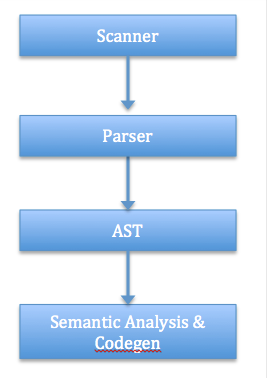
\includegraphics[width=9cm, height=7.5cm]{arch.png} 
     \caption{\label{lb}MatCab Architecture} 
\end{figure}
\subsection{Scanner}
The scanner is used to tokenize the input file into token streams. The scanner will eliminate all kinds of useless tokens, such as tabs, white spaces, tabs, etc, and will raise an error if the scanner meets an illegal token. We used ocamllex to build the scanner.

\subsection{Parser}
The parser accepts the token stream generated by the scanner and parses it to build an AST. If the input token stream does not meet the requirements of the predefined syntax, it will raise an error. We used ocamlyacc to build the parser.

\subsection{AST}
The abstract syntax tree eliminates some unnecessary parts of elements at the parsing phase to the rest compiling job easier.  Figure 4 is the type checking list.

\subsection{Compiler}
The compiler accepts an AST and recursively traverse each node of it, translating it into Java code while doing the type checking at the same time. If there is something wrong, it will raise an error.   

\begin{table}
\centering
\caption{Type checking list}
\begin{tabular}{|c|} \hline
Accessing an undeclared variable \\ \hline
Invoking an undefined function \\ \hline
The arguments of a function call does not match the formal list\\ \hline
Calculating the determinant of a non-matrix variable \\ \hline
Calculating the trace of a non-matrix variable \\ \hline
Returning the submatrix of a non-matrix variable \\ \hline
Returning the area sum of a non-matrix variable \\ \hline
Returning the convolution of a non-matrix variable \\ \hline
Returning the inverse of a non-matrix variable \\ \hline
Returning the transpose of a non-matrix variable \\ \hline
Accessing an non-integer index of a matrix \\ \hline
Assigning a non-matrix variable to a matrix \\ \hline
Adding/Substrcting an integer to(from) a matrix \\ \hline
No entry function \\ \hline
The entry function has arguments \\ \hline
\end{tabular}
\end{table}


%-------------
%	Test cases
%----------------
\section{Test Plan}
Our project can be roughly divided into two phases: 
1. The design and implementation of the parser and Ast\\
2. The construction of the compiler (also translater). 

Tests were involved in both phases and every single feature was tested with a corresponding test file. 

The construction of the compiler did not start until we had run sufficient tests on our parser and ast and fixed all detected bugs. Started from here, new test file would be added into our test suite when our compiler got a new functionality. 

Automation was used during our tests. A bash script was written to processing all test files inside the test suite. The direct result and intermediate java source code was recoded for possible future inspection. 
Our Test Suites was divided into several sub suites, each focused on one domain of our program. Here is a list of all the sub suites, with self-explanatory names: basic comprehensive, expr, func, stmt, var

\subsection{basic}
This suite tested the most basic functionalities and top level structure of our language. 
Sample program: Basic5.mcb 
This program aimed to test: variable and function declaration, both local and global, the return statement, the type checking of return value, and the recognition of the entry() function.  

\begin{lstlisting}
int entry() {
    int a;
    int b;
}

float f1;
float foo(int bar) {
    return 0;
}

int baz;

\end{lstlisting}

\subsection{expr}
This suite tested the parsing and implementation of normal and nested expressions. The tests of arithmetic calculations and matrix operations were also include in this suite.
Sample: expr10.mcb  
This program mainly tested matrix initialization, which was achieved through nested expressions. Same for the print function. 
\begin{lstlisting}
int entry() {
    int a;
    floatMat b;
    floatMat d;
    
    Init b[3][3];
    b = [[ 1,2,3?4,5,6?9,8,7]];
    Init d[3][3];
    d = [[ 10, 0, 30 ? 44, 2, 92 ? 3, 49, 72 ]];
    b = b * 11;
    print(b[2][2]);
    d = d ** b;
    print(d[1][1]);
}
\end{lstlisting}

\subsection{func}
This suite basically tested the function call and declaration. 
Sample: fun4.mcb
This program tested the call and declaration of the foo function, which returns an element of a matrix. Note that foo is called inside the call to print as parameter. 
\begin{lstlisting}
float foo(floatMat A, int x, int y) {
    return A[x][y];
}

int entry() {
    floatMat B;
    int xx;
    int yy;
    xx = 3;
    yy = 4;
    Init B[10][10];
    B[1][1] = 9;
    print(foo(B, xx, yy) + 33);
}

\end{lstlisting}


\subsection{stmt}
This suite tested the parsing and implementation of statements
Sample: stmt8.mcb
This program tested the ``for'' loop, which is a statement. 
\begin{lstlisting}
int entry() {
    int a;
    for (a = 0; a < 10; a = a + 1)
        print(333);
}
\end{lstlisting}



\subsection{var}
This suite tested the initialization and declaration of variables
Sample: var9.mcb
This program tested the initialization of a matrix. Note that we assigned Mat A with an illegal matrix expression, which has inconsistent number of elements on each row. So we were expecting an error to be thrown here. 
\begin{lstlisting}
int entry() {
    floatMat A;
    Init A[3][5];
    A = [[ 1, 2 ? 3, 4, 5 ]];
}
\end{lstlisting}

\subsection{comprehensive}
This suite tested many features our language as a whole. Test programs in this suite were relatively complicated and did some actual stuff. 
Sample: fib.mcb
This program found and printed out the fifth Fibonacci number. Recursive call, if-else flow, along with some basic features were tested. 
\begin{lstlisting}
int fib(int n) {
    int tmp;
    if (n == 1)
        return 1;
    endif;
    
    if (n == 2)
        return 1;
    endif;
    
    if (n >= 3)
    {
        tmp = fib(n-1) + fib(n-2);
        return tmp;
    }
    endif;    
    return 0;
}

int entry() {
    print(fib(5));
}


\end{lstlisting}


%----------------
%	Lesson learned
%-----------------
\section{Lesson Learned}
This section gives the lessons learned by each member.

\subsection{Cheng Xiang}
Originally I was quite optimistic about our project. Because it seems that nobody, as far as I know at least, had ever developed language that exploited the simplicity and beauty of Matlab-like matrix manipulation syntax, and exploited the concurrable nature of many matrix calculations to accelerate the calculation process at the same time. However our development didn’t go quite smoothly. At last we submitted a runnable compiler using syntax close to Matlab, but did not produce CUDA code. Being the “leader” of this project team, I thought there are several reasons for this.

First of all, the team leader has to be able to do the time management wisely. It would be best if all the team members could agree on a fixed time in each week to sit down and work something serious out. Secondly, appropriate milestones and timeline should be set up by the team leader. We got stuck at developing parser and constructing the AST for quite long a time. This is the primary reason we didn’t choose to output CUDA executable code and selected relatively simpler Java code instead. And last, the team member should always be good at communicate with team members. He/She should play as a role model and encourage other team members to steadily move on along the path of development.
Advice for future teams

Implementing a translator or compiler for a given language is comparably simple. The difficult and fun part lies in developing your own language. With so many long-existing languages it may seem quite hard to come up with a brilliant idea. Even you think you get an extraordinary idea, keep in mind that idea is worthless unless it is carried out. Try to group up with people with different specialties and academic backgrounds, and consult friends (especially those PhD ones working in areas besides computer science)  during the design of your own language.

\subsection{Tianchen Yu}
For me, the most valuable lesson learned during our project is that coordination among team members can greatly improve the team efficiency. We have a very clear role for each member of our team. After the parser and ast were done, everybody did their tasks concurrently. And we knew who to ask if we encountered a problem. This made the second phase of our project went smoothly and fast. We did a lot of thing within only a few days. 

Also, it is much better to find a rather long time period when everybody is available, ideally a whole day. In this way the whole team would be more devoted into the tasks. Having some one leaving in the middle of a meeting sometimes diminish the passion of other team members. 

Advice for Future Teams:Spread the task evenly throughout the semester. Don’t push everything to the very last week. The parser and ast should be done around mid term so you will have plenty of time to implement the rest and do tests without having to cut off some features could be pretty awesome. 

\subsection{Ran Yu}
Although I have implemented a compiler in my undergraduate study, MatCab is a really different one. Thinking in the O'Caml way is such a different experience for me.
 
Except Functional language, I learned in detail how the AST, scanner, parser and compiler are worked together to translate a programming language into executable. It is much more hard than I expected, but I am very glad that our team work together and make it.

Also I learned how to design unit test that discover all kind of dark corner and fix the problem with teammates.

Last but not least, the project teach me a lot in team working. How to deal with each other and how to make the project developed more efficient. In our project, everyone of us gave the best effort to implement the compiler. 

\subsection{Yu Qiao}
The first lesson I learnt is start early, although this has been repeatedly stated by so many times by different teams. OCaml is a language that is very difficult to command, and it requires far more time than expected to write just a few lines of code. Starting early means getting a deep understanding of OCaml and thus make the following work smoothly. 

The second lesson is to define LRM accurately first. We did not come up with a crystal clear LRM at first, and that proves to be a mistake. We had to revise the parser and AST again and again when doing the real coding, which is a great waste of time. 

The third lesson is to resolve the technical risk at the very begging. We failed to generate CUDA code because we could not finish it in a very short time. Learning something new is always time-consuming, and the best way is to let someone resole this risk at first. 



%----------------------------------------------------------------------------------------
%	BIBLIOGRAPHY
%----------------------------------------------------------------------------------------

\begin{thebibliography}{99} % Bibliography - this is intentionally simple in this template

\bibitem[Dennis M. Ritchie, 1973]{DMR:1973dg}
Dennis M. Ritchie (1973).
\newblock C Reference Manual.
\newblock {\em Bell Telephone Laboratories}

\bibitem[Jeremy, Robert, Kevin and Yongxu, 2011]{JRKY:2011dg}
Jeremy Andrus and Robert Martin and Kevin Sun and Yongxu Zhang (2011).
\newblock CLAM: The Concise Linear Algebra Manipulation Language.
\newblock {\em Columbia University}

\end{thebibliography}

%----------------------------------------------------------------------------------------

\end{document}
